\chapter{Motivación y antecedentes}
\label{ch:antecedentes}

En la actualidad, existe un problema a la hora de encontrar un equilibrio entre la oferta de plazas disponibles y la demanda real de pasajeros en el transporte ferroviario. Esto supone un gran reto operativo para las empresas que ofertan servicios ferroviarios, dado que la venta de billetes debe ajustarse a la capacidad de cada tren, intentando evitar tanto una saturación de los servicios, como un bajo aprovechamiento de los mismos. Este problema surge debido a la liberalización y creciente competitividad en los mercados ferroviarios, especialmente en Europa, donde se ha fomentado la competencia entre distintos operadores ferroviarios con la búsqueda de un espacio ferroviario europeo único. Para abordar este problema, investigadores de la Universidad de Castilla-La Mancha, de los grupos ORETO y MAT de la Escuela Superior de Informática han desarrollado \acrfull{ROBIN}~\cite{delCastilloHerrera2024ROBIN} que consiste en un simulador destinado a modelar la movilidad de pasajeros en entornos ferroviarios en los que exista una competencia entre los diferentes operadores. 

\acrshort{ROBIN} adopta un enfoque completamente microscópico, simulando pasajero a pasajero y asiento a asiento. Para cada pasajero potencial, el simulador evalúa todas las alternativas de servicio disponibles (teniendo en cuenta para ello horarios, tipos de asiento y condiciones comerciales) y determina la elección final de cada usuario según reglas de decisión basadas en utilidad y aleatoriedad. De este modo, permite cuantificar con detalle la demanda atendida, los pasajeros que no viajan por falta de plazas y los flujos de ocupación en cada tramo de la red.

La arquitectura de \acrshort{ROBIN} está dividida en tres componentes principales: un módulo de oferta que procesa la información de los servicios disponibles (obtenida generalmente mediante \textit{scraping} de fuentes como la web de Renfe), un módulo de demanda que genera perfiles de usuario y distribuciones de viaje, y un núcleo de simulación que coordina ambas entradas para ejecutar el escenario diario. Al finalizar, todos los datos de salida (ocupaciones, rechazos de demanda y métricas de rendimiento) se exportan automáticamente en formato \acrshort{CSV} para su posterior análisis.

Gracias a su diseño modular y parametrizable, \acrshort{ROBIN} facilita la experimentación con distintos escenarios de mercado: variaciones en los hábitos de viaje, ajustes de precios, incorporación de nuevos operadores o cambios en la infraestructura. Esto convierte al simulador en una herramienta estratégica para evaluar el impacto de políticas de liberalización, estrategias de precios y planes de capacidad antes de su puesta en marcha real.

\begin{figure}[H]
\centering
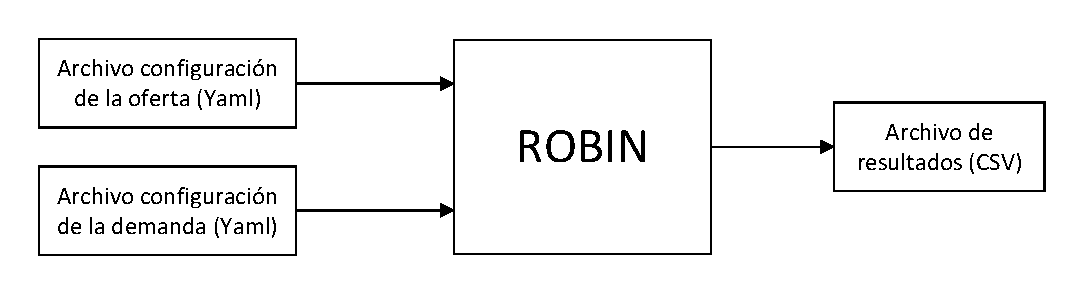
\includegraphics[width=.9\textwidth]{fig/Diagramas/Esquema ROBIN.pdf}
\caption{Esquema de entrada y salida de archivos actual de \acrshort{ROBIN}}
\label{fig:esquemaROBIN}
\end{figure} 

\acrshort{ROBIN} emplea archivos en formato \acrfull{Yaml} para cargar los datos de la oferta y la demanda para realizar las simulaciones, y genera como salida ficheros \acrfull{CSV} con los resultados de las mismas. El manejo de estos archivos puede resultar tedioso debido a la gran cantidad de información que se ha de manejar para realizar la simulación con \acrshort{ROBIN}. Esto debido a que han de analizarse, para cada pasajero modelado en el sistema, todos los posibles asientos de cada servicio de forma individual. 

Concretamente, el programa emplea dos archivos \acrshort{Yaml} como entrada de datos: un archivo con la información de la oferta en el mercado que se va a simular y un archivo con los patrones de usuario y los patrones de demanda esperados para el día que se desea estudiar (Figura \ref{fig:esquemaROBIN}). La información de la oferta, que posteriormente se usará en el simulador, proviene de una herramienta de extracción de datos web (\textit{scraper}) empleada en diferentes páginas, como por ejemplo, la página de venta al público de \textit{Renfe}\footnote{Web de venta de billetes de Renfe: \href{https://www.renfe.com/es/es}{https://www.renfe.com/es/es}}. De esta forma, se recopilan los datos de todas las estaciones dentro del sistema ferroviario español. Este programa genera diferentes archivos con datos sobre la oferta, dependiendo del corredor español al que pertenecen los servicios y de las fechas de los mismos. Finalmente, al acabar la simulación, se genera un archivo \acrshort{CSV} con los resultados obtenidos. 

%\textbf{TEMA: REESCRIBIR, VA UN POCO RELACIONADA CON EL COMENTARIO ANTERIOR} En este contexto, se vislumbra la necesidad de contar con un sistema que ayude a realizar el manejo de dichos archivos. Por ello, este \acrfull{TFG} se ha centrado en la creación de una herramienta para gestionar los ficheros de configuración, en formato \acrshort{Yaml}, y los ficheros de resultados, en formato \acrshort{CSV} asociados a \acrshort{ROBIN}.

%De esta manera, todos los archivos, tanto de entrada como de salida, que emplea \acrshort{ROBIN} se encontrarían almacenados en un único lugar, eliminando la necesidad de organizar los ficheros a mano y sería la herramienta la que se encargaría de la gestión de dichos archivos.

Los archivos \acrshort{Yaml} tienen un acceso muy rápido para pequeños volúmenes de datos, pero cuando el volumen de datos aumenta, se vuelve más lento, debido a que hay que cargar y procesar el archivo completo en memoria para poder acceder a los datos. Esto también deriva en un problema de escalabilidad, ya que para grandes volúmenes de datos, habría que procesar un archivo que contiene mucha información, lo que puede derivar en demoras a la hora de cargar el archivo en memoria. Por todo esto, las bases de datos relacionales son una alternativa al aportar una serie de ventajas:
\begin{itemize}
    \item Son rápidas y eficientes a la hora de manejar grandes volúmenes de datos debido a que la información se procesa por bloques.
    \item Tienen la información bien organizada y previenen la duplicidad de información.
    \item Permiten consultas sobre los resultados obtenidos de una forma más sencilla y eficiente que en el archivo \acrshort{CSV}.
\end{itemize}

En este contexto, este \acrshort{TFG} se centra en la creación de una herramienta para gestionar los ficheros de entrada de datos de la oferta y de la demanda, en formato \acrshort{Yaml}, y los ficheros de resultados, en formato \acrshort{CSV} asociados a \acrshort{ROBIN} utilizando bases de datos relacionales. De esta forma, la información de los archivos de entrada y salida que emplea \acrshort{ROBIN} en la actualidad se almacenará en 3 bases de datos, una para cada tipo de archivo, para un mejor manejo y tratamiento de la información, siendo la herramienta desarrollada la que se encargue de la gestión de dichos archivos. De esta manera, toda la información relacionada con los diferentes archivos, tanto de entrada como de salida, quedará almacenada en un único punto. Además, se pretende diseñar y desarrollar una interfaz para el manejo de los datos de entrada y salida, lo que permitirá realizar consultas sobre los datos manejados y generados en las simulaciones. Esto es de gran utilidad dentro de este entorno. La Figura \ref{fig:esquemaROBINConDB} muestra la nueva estructura de trabajo de \acrshort{ROBIN}, en la que se muestra cómo se generarán los archivos \acrshort{Yaml} desde la información de las bases de datos. Además, los resultados de las simulaciones se almacenarán en una base de datos de salida que permitirá realizar consultas sobre éstos.

\begin{figure}[H]
\centering
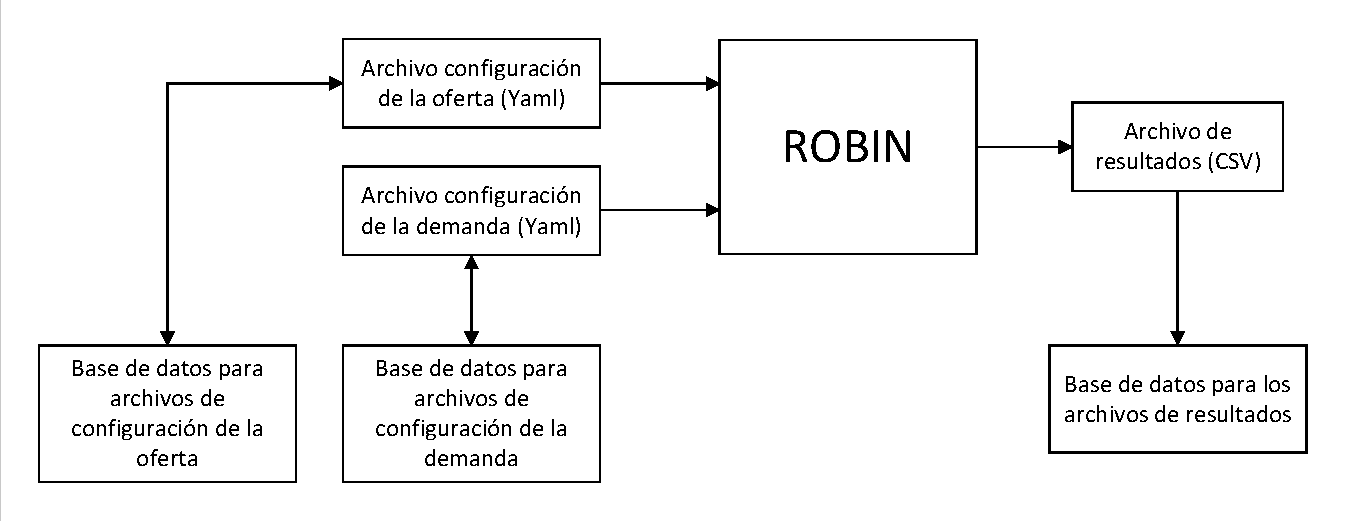
\includegraphics[trim={0.2cm, 0.4cm, 0.2cm, 0.4cm}, clip, width=.9\textwidth]{fig/Diagramas/Esquema ROBIN con base de datos.pdf}
\caption{Esquema de entrada y salida de archivos de \acrshort{ROBIN} tras la realización del \acrshort{TFG}}
\label{fig:esquemaROBINConDB}
\end{figure}

Para la creación de sistemas de gestión de archivos, pueden emplearse diversos lenguajes de programación como C, Java, Python, etc. Uno de los más útiles, en este contexto, para la programación e implementación de este gestor, es el lenguaje Python~\cite{Python}~\cite{Romano2015}~\cite{VanHattem2016} debido a que se trata de un lenguaje fácil de aprender y cuenta con una extensa cantidad de librerías, lo que permite una gran variedad de opciones para el desarrollo. Dentro de la gran cantidad de librerías de las que dispone Python, cabe recalcar algunas que son especialmente útiles para los objetivos de este TFG, como son: 

\begin{itemize} 
    \item \textbf{PyYAML~\cite{PyYaml}~\cite{yaml_quick_start_2019}~\cite{wittmann_mastering_yaml_2023}:} Esta librería permite la lectura y creación de archivos en formato \acrshort{Yaml}. Permite a Python obtener datos de los ficheros con formato \acrshort{Yaml} al transformar los datos contenidos en este a estructuras que puedan ser utilizadas en Python como listas o diccionarios. También permite transformar estas estructuras al formato empleado por los ficheros \acrshort{Yaml}.
    
    \item \textbf{sqlite3~\cite{SQLite3}~\cite{Python_SQLite3}~\cite{learn_sqlite_python_2019}:} Se trata de una interfaz DB-API 2.0\footnote{Define un conjunto de métodos y convenciones para acceder de forma uniforme a distintas bases de datos desde Python.} para trabajar con bases de datos SQLite desde Python. Esto permite la creación y edición de bases de datos, así como, la realización de consultas a estas bases de datos.
    
    \item \textbf{csv~\cite{Python_CSV}~\cite{martelli_modern_python_cookbook_2019}:} Esta librería se trata de un módulo nativo de Python para leer y escribir archivos \acrshort{CSV}.

    \item \textbf{Tkinter~\cite{Tkinter}~\cite{Meier2017}~\cite{moore_tkinter_2021}:} Se trata de una biblioteca estándar de Python para interfaces gráficas de usuario (GUI). Permite construir ventanas, menús, formularios y controles sin necesidad de instalar dependencias externas.
\end{itemize}

Otra herramienta que cabe mencionar es SQLiteStudio~\cite{SQLiteStudio} que resulta muy útil para la creación, edición y visualización de bases de datos que empleen SQLite como motor de base de datos. Además, permite interaccionar con las bases de datos conectadas a la aplicación mediante el uso de sentencias con lenguaje \acrfull{SQL}. 